\documentclass[12pt,a4paper]{report}

\usepackage{styles/dolgozat}

\usepackage{listings}
\usepackage{styles/cpp}
\usepackage{styles/python}

\usepackage{hyperref}

\begin{document}

\pagestyle{empty} %a címlapon ne legyen semmi=empty, azaz nincs fejléc és lábléc

% A Miskolci Egyetem címere
{\large
\begin{center}
\vglue 1truecm
\textbf{\huge\textsc{Szakdolgozat}}\\
\vglue 1truecm

\includegraphics[width=4.8truecm, height=4truecm]{images/me_logo.png}\\
\textbf{\textsc{Miskolci Egyetem}}
\end{center}}

\vglue 1.5truecm %függõleges helykihagyás

% A szakdolgozat címe, akár több sorban is
{\LARGE
\begin{center}
\textbf{A szakdolgozat címe}
\end{center}}

\vspace*{2.5truecm}
% A hallgató neve, évfolyam, szak(ok), a konzulens(ek) neve
{\large
\begin{center}
\begin{tabular}{c}
\textbf{Készítette:}\\
Szakdolgozó Neve\\
Programtervező informatikus
\end{tabular}
\end{center}
\begin{center}
\begin{tabular}{c}
\textbf{Témavezető:}\\
Piller Imre
\end{tabular}
\end{center}}
\vfill
% Keltezés: Hely, év
{\large
\begin{center}
\textbf{\textsc{Miskolc, 2020}}
\end{center}}

\newpage


\newpage

\pagestyle{empty}

%Feladatkiiras
\begin{flushleft}
\textsc{\bfseries Miskolci Egyetem}\\
Gépészmérnöki és Informatikai Kar\\
Alkalmazott Matematikai Intézeti Tanszék\hspace*{4cm}\hfil \textbf{Szám:}
\end{flushleft}
\vskip 0.5cm
\begin{center}
\large\textsc{\bfseries Szakdolgozat Feladat}
\end{center}
\vskip 0.5cm
Szakdolgozó Reisz Ákos (FZ3S16) mérnökinformatikus jelölt részére.\newline

\noindent\textbf{A szakdolgozat tárgyköre:} optimalizáció, szimuláció, étterem, kiszállítás\newline

\noindent\textbf{A szakdolgozat címe:} Éttermi kiszállítás szimulációja és optimalizációja\newline

\noindent\textbf{A feladat részletezése:}

Az éttermi rendelések kiszállításánál megjelenő optimalizálási problémák szimulációja és vizsgálata. Az optimalizálás célja, hogy minél több megrendelést, minél rövi\-debb idő alatt, minél kisebb költséggel lehessen teljesíteni.

A dolgozat az egyszerűbb problémáktól az egyre valószerűbbek (így komplikáltabbak) felé haladva vizsgálja az optimalizálási problémák modelljét, lehetséges megoldási módjait. A legegyszerűbb esetnek az egy futár, egy étterem és egy kiszállítás esete tekinthető. Egy fokkal bonyolultabb változatban több kiszállítást is számításba kell venni, majd ezt követően a több étterem és több futár esetét is célszerű megvizsgálni.

Az optimalizálás során több célfüggvényt is érdemes megvizsgálni. Ilyen lehet pél\-dául a kiszállítási idő vagy az egy kiszállításhoz tartozó megtett út minimalizálása.
A szimuláció és az optimalizálás Python programozási nyelv segítségével készül. Az algoritmusok vizsgálatához a különféle paraméterezések vizsgálata Jupyter munkafüze\-tek\-ben történik. Az elkészült algoritmusok egy Python függvénykönyvtárba kerülnek. A működés helyességét az elkészített egységtesztek támasztják alá.

\vfill

\noindent\textbf{Témavezető:} Piller Imre (egyetemi tanársegéd) \newline

% \noindent\textbf{Konzulens(ek):} (akkor kötelezõ, ha a témavezetõ nem valamelyik matematikai tanszékrõl való; de persze lehet egyébként is)\newline

\noindent\textbf{A feladat kiadásának ideje:}\newline

%\noindent\textbf{A feladat beadásának határideje:}

\vskip 2cm

\hbox to \hsize{\hfil{\hbox to 6cm {\dotfill}\hbox to 1cm{}}}

\hbox to \hsize{\hfil\hbox to 3cm {szakfelelős}\hbox to 2cm{}}

\newpage

\vspace*{1cm}  
\begin{center}
\large\textsc{\bfseries Eredetiségi Nyilatkozat}
\end{center}
\vspace*{2cm}  

Alulírott \textbf{Reisz Ákos}; Neptun-kód: \texttt{FZ3S16} a Miskolci Egyetem Gépészmérnöki és Informatikai Karának végzős Mérnökinformatikus szakos hallgatója ezennel büntetőjogi és fegyelmi felelősségem tudatában nyilatkozom és aláírásommal igazolom, hogy \textit{Éttermi kiszállítás szimulációja és optimalizációja}
című szakdolgozatom saját, önálló munkám; az abban hivatkozott szakirodalom
felhasználása a forráskezelés szabályai szerint történt.\\

Tudomásul veszem, hogy szakdolgozat esetén plágiumnak számít:
\begin{itemize}
\item szószerinti idézet közlése idézőjel és hivatkozás megjelölése nélkül;
\item tartalmi idézet hivatkozás megjelölése nélkül;
\item más publikált gondolatainak saját gondolatként való feltüntetése.
\end{itemize}

Alulírott kijelentem, hogy a plágium fogalmát megismertem, és tudomásul veszem, hogy
plágium esetén szakdolgozatom visszautasításra kerül.

\vspace*{3cm}

\noindent Miskolc, \hbox to 2cm{\dotfill} .év \hbox to 2cm{\dotfill} .hó \hbox to 2cm{\dotfill} .nap

\vspace*{3cm}

\hspace*{8cm}\begin{tabular}{c}
\hbox to 6cm{\dotfill}\\
Hallgató
\end{tabular}



\newpage

\noindent 1.

\begin{tabular}{cl}
&szükséges (módosítás külön lapon) \\
A szakdolgozat feladat módosítása& \\
& nem szükséges\\
&\\
\hbox to 4cm{\dotfill}&\multicolumn{1}{c}{\hbox to 5cm{\dotfill}}\\
dátum& \multicolumn{1}{c}{témavezető(k)}
\end{tabular}
\vskip1.5mm

\noindent 2. A feladat kidolgozását ellenőriztem:

\vskip1.5mm

\begin{tabular}{l@{\hspace*{4cm}}l}
témavezető (dátum, aláírás):& konzulens (dátum, aláírás):\\
\dotfill&\dotfill\\
\dotfill&\dotfill\\
\dotfill&\dotfill
\end{tabular}

\vskip1.5mm

\noindent 3. A szakdolgozat beadható:

\vskip1.5mm

\begin{tabular}{@{\hspace*{1.3cm}}c@{\hspace*{2.1cm}}c}
\hbox to 4cm{\dotfill}&\multicolumn{1}{c}{\hbox to 5cm{\dotfill}}\\
dátum& \multicolumn{1}{c}{témavezető(k)}
\end{tabular}

\vskip1.5mm

\noindent 4.
\begin{tabular}[t]{@{}l@{\hspace*{1mm}}l@{\hspace*{1mm}}l@{}}
A szakdolgozat& \hbox to 3.5cm{\dotfill} &szövegoldalt\\
              & \hbox to 3.5cm{\dotfill} &program protokollt (listát, felhasználói leírást)\\
              &\hbox to 3.5cm{\dotfill}   &elektronikus adathordozót (részletezve)\\
              &\hbox to 3.5cm{\dotfill} & \\
              &\hbox to 3.5cm{\dotfill} &egyéb mellékletet (részletezve)\\
              &\hbox to 3.5cm{\dotfill} &\\
\end{tabular}
\newline tartalmaz.

\vskip1.5mm

\begin{tabular}{@{\hspace*{1.3cm}}c@{\hspace*{2.1cm}}c}
\hbox to 4cm{\dotfill}&\multicolumn{1}{c}{\hbox to 5cm{\dotfill}}\\
dátum& \multicolumn{1}{c}{témavezető(k)}
\end{tabular}

\noindent 5.

\begin{tabular}{ll}
&bocsátható\\
A szakdolgozat bírálatra& \\
& nem bocsátható\\
\end{tabular}

\vskip1.5mm

\noindent A bíráló neve: \hbox to 8cm{\dotfill}

\vskip4mm

\begin{tabular}{@{\hspace*{1.3cm}}c@{\hspace*{2.1cm}}c}
\hbox to 4cm{\dotfill}&\multicolumn{1}{c}{\hbox to 5cm{\dotfill}}\\
dátum& \multicolumn{1}{c}{szakfelelős}
\end{tabular}

\noindent 6.
\begin{tabular}[t]{@{}l@{\hspace*{1mm}}l@{\hspace*{1mm}}l@{}}
A szakdolgozat osztályzata& &\\
&a témavezető javaslata:& \hbox to 3cm{\dotfill}\\
&a bíráló javaslata:& \hbox to 3cm{\dotfill}\\
&a szakdolgozat végleges eredménye:& \hbox to 3cm{\dotfill}
\end{tabular}

\vspace*{4mm}

\noindent Miskolc, \hbox to 4.5cm{\dotfill} \hspace*{2.5cm}
\begin{tabular}[t]{cc}
\hbox to 6cm{\dotfill}\\
a Záróvizsga Bizottság Elnöke
\end{tabular}


\cleardoublepage
\pagenumbering{gobble}
\tableofcontents
\cleardoublepage
\pagenumbering{arabic}

\newpage

\pagestyle{fancy}

\Chapter{Bevezetés}

A fejezet célja, hogy a feladatkiírásnál kicsit részletesebben bemutassa, hogy miről fog szólni a dolgozat.
Érdemes azt részletezni benne, hogy milyen aktuális, érdekes és nehéz probléma megoldására vállalkozik a dolgozat.

Ez egy egy-két oldalas leírás.
Nem kellenek bele külön szakaszok (section-ök).
Az irodalmi háttérbe, a probléma részleteibe csak a következő fejezetben kell belemenni.
Itt az olvasó kedvét kell meghozni a dolgozat többi részéhez.

% \Chapter{Koncepció}

\Section{A fejezet célja}

Ez a fejezet még nem a saját eredményekkel foglalkozik, hanem bemutatja, mi a problémakör, milyen módszerekkel, milyeneredményeket sikerült elérni eddig másoknak.

A hivatkozások jelentős része ehhez a fejezethez szokott kötődni.
(Egy hivatkozás például így néz ki \cite{coombs1987markup}.)
Itt lehet bemutatni a hasonló alkalmazásokat.

\Section{Tartalom és felépítés}

A fejezet tartalma témától függően változhat. Az alábbiakat attól függően különböző arányban tartalmazhatják.
\begin{itemize}
\item Irodalomkutatás. Amennyiben a dolgozat egy módszer kidolgozására, kifejlesztésére irányul, akkor itt lehet részletesen végignézni (módszertani vagy időrendi bontásban), hogy az eddigiekben milyen eredmények születtek a témakörben.
\item Technológia. Mivel jellemzően kutatásról vagy szoftverfejlesztésről van szó, ezért annak a jellemző elemeit, technikai részleteit itt kell bemutatni.
Ez tehát egy módszeres bevezetés ahhoz, hogy ha valaki nem jártas a témakörben, akkor tudja, hogy a dolgozat milyen aktuálisan elérhető eredményeket, eszközöket használt fel.
\item Piackutatás. Bizonyos témáknál új termék vagy szolgáltatás kifejlesztése a cél.
Ekkor érdemes annak alaposan utánanézni, hogy aktuálisan milyen eszközök érhetők el a piacon.
Ez szoftverek esetében a hasonló alkalmazások bemutatását, táblázatos formában történő összehasonlítását jelentheti.
Szerepelhetnek képek és észrevételek a viszonyításként bemutatott alkalmazásokhoz.
\item Követelmény specifikáció. Külön szakaszban érdemes részletesen kitérni az elkészítendő alkalmazással kapcsolatos követelményekre.
Ehhez tartozhatnak forgatókönyvek (\textit{scenario}-k).
A szemléletesség kedvéért lehet hozzájuk képernyőkép vázlatokat is készíteni, vagy a használati eseteket más módon szemléltetni.
\end{itemize}

\Section{Amit csak említés szintjén érdemes szerepeltetni}

Az olvasóról annyit feltételezhetünk, hogy programozásban valamilyen szinten járatos, és a matematikai alapfogalmakkal sem ebben a dolgozatban kell megismertetni.
A speciális eszközök, programozási nyelvek, matematikai módszerekk és jelölések persze jó, hogy ha említésre kerülnek, de nem kell nagyon belemenni a közismertnek tekinthető dolgokba.

\Chapter{A kiszállítási problémák általános modelljei}

A kiszállítási probléma vizsgálatához először annak általános modelljét kell megadni.
A vizsgált absztrakciós szintén a modell három alapvető eleme az étterem, a futár és a rendelés/kiszállítás helye (\ref{fig:generalModel}. ábra).

\begin{figure}[h!]
	\centering
	
\includegraphics[scale=0.5]{images/complexModel.png}
	\caption{Éttermi rendelés modelljének három fő tényezője, úgy mint az étterem, a futár és a rendelés helye (képek forrása: \cite{Image1}, \cite{Image2}, \cite{Image3})}
	\label{fig:generalModel}
\end{figure}

Az absztrak modellek nyilván nem írják le teljes részletességében a problémákat.
Jelen esetben a következőket várjuk el a felírt modelltől.
\begin{itemize}
	\item Az éttermeket és a kiszállítások helyét pontszerűnek tekinti.
	\item Szóhasználatot illetően azt feltételezzük, hogy a kiszállítás egyetlen városon belül történik. (Ez a matematikai modell szempontjából nem lényegi megkötés, de a problémák leírását egyszerűsíti.)
	\item Nem feltételezi, hogy a futárnak lenne kapacitás, üzemanyag, vagy bármilyen hasonló jellegű limitációja.
	\item A kiszállítások bejárási sorrendjére vonatkozóan azon túlmenően, hogy mindegyiket be kell járnia a futárnak, külön nincsen. Az optimalizálási probléma eredményeként várjuk, hogy mi az optimális sorrend.
	\item A kiszállítás pontos idejére vonatkozóan nincs korlátozó tényező. A felvázolt modell az időt csak a megtett út függvényében képes tekinteni.
	\item Nem tekintünk a modell részének semmilyen közbeiktatott változást (például a rendelés lemondását) vagy egyéb problémát (például a futár járművének meghibásodását, kiszállítással kapcsolatos problémát).
\end{itemize}
Ezen egyszerűsítések mellett is láthatjuk majd, hogy igen változatos esetekben, komoly optimalizálási problémák megoldására lesz szükség.

\Section{A probléma modelljének lehetséges esetei}

A szóbajöhető lehetőségek egyszerűbb áttekinthetősége érdekében adjunk meg hármasokat, melyekben az elemek az éttermek, futárok és kiszállítások számosságára vonat\-koznak.
A számosság itt lehet jelenthet egyet vagy többet. Előbbit $1$-el, utóbbit pedig $*$-al fogjuk jelölni.
Ezen jelölésrendszert használva összesen 8 lehetséges hármas adódna, úgy mint
\[
(1, 1, 1),
(1, 1, *),
(1, *, *),
(1, *, 1),
(*, 1, *),
(*, *, 1),
(*, 1, 1),
(*, *, *).
\]
A következő szakaszban azt vizsgáljuk és indokoljuk meg, hogy melyek azok az esetek, amelyekkel ezek közül nem érdemes foglalkozni.

\Section{Figyelmen kívül hagyott és vizsgált esetek}

\begin{itemize}
\item \textit{Egy étterem, több futár, egy kiszállítás}:
Nincs értelme vizsgálni, mivel egyetlen kiszállításhoz elegendő csak egy futár.
\item \textit{Több étterem, egy futár, egy kiszállítás}: Egy kiszállításnak szükségszerűen egy adott étteremből kell indulnia, tehát ez az eset nem értelmezhető.
\item \textit{Több étterem, több futár, egy kiszállítás}: Hasonlóan az előző esethez, nem tudjuk értelmezni, mert egy kiszállításhoz egyértelműen tartozik egyetlen étterem és egyetlen futár.
\end{itemize}

Az említett eseteket kihagyva az optimalizálási problémákat a következőkre tudjuk megadni:
\begin{itemize}
\item egy étterem, egy futár, egy kiszállítás,
\item egy étterem, egy futár, több kiszállítás,
\item több étterem egy futár, több kiszállítás,
\item egy étterem, több futár, több kiszállítás,
\item több étterem, több futár, több kiszállítás.
\end{itemize}
Az így adódó optimalizálási problémákat és azok lehetséges megoldásait a dolgozat a további fejezetekben mutatja be.

\Section{A város reprezentálása}

Úgy tekintjük, hogy az éttermek és a kiszállítások helyei is egy városon belül vannak.
A modell síkban gondolkozik, tehát egy étteremhez és egy kiszállítási helyhez is egy $(x, y) \in \mathbb{R}^2$ koordináta tartozik.

A közlekedési hálózat modellje egy gráf, amely azt adja meg, hogy melyik pontból melyikbe lehet eljutni.
Egy kiszállítás útvonala tehát ezen pontok közötti szakaszok sorozatának tekinthető, melyen az éttermek és a kiszállítási helyek is egy-egy pontot jelentenek.

\Chapter{Egy étterem, egy futár, egy kiszállítás esete}

\Section{A probléma megfogalmazása}

Ebben az esetben egy étterem található a városban, amelyből csak egy futár szállít ki mindig csak egy címre.
Bonyolultságát tekintve a legrövidebb utat kell megtalálni két pont között feltételezve azt, hogy egy pontból a másikba nem lehet közvetlenül eljutni, hanem más pontokat érintve csak. Ezáltal egy gráf élein kell végigmenni és közben keresni a legrövidebb a legrövidebb távot. Az optimális út meghatározása után venni kell ezen út hosszúnak kétszeresét, mivel a futár a szállítást követően vissza kell, hogy térjen az étterembe. Két pont közötti hossz meghatározására kiválló példa az egyik leginkább ismert algoritmus az A* algoritmus.

\begin{figure}[h!]
\centering
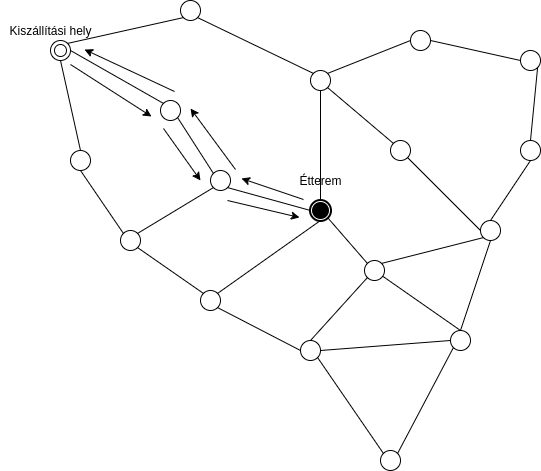
\includegraphics[scale=0.5]{images/Astar.png}
\caption{Egy étterem, egy futár, egy kiszállítás modellje}
\label{fig:model1}
\end{figure}

\Section{A probléma megoldása}

A* algoritmus

Az eljárásban a kiértékelő függvényünk a heurisztikus fügvény. Maga a fő ciklus minden iterációjánál az A*-nak meg kell határoznia az általala kiterjesztendő utat. A szakasz költségét és a célhoz érésnek költségét veszi figyelembe. Így az A* meghatározza az f(n) = g(n) + h (n) függvényt minimalizáló utat. n-nel jelölik a következő úton található csúcsot, ezáltal g(n) a kezdőpontból n-ig tartó út költsége. A heurisztikus függvényt h(n)-nel azonosítható, ez pedig nem más mint az n-től a célig vezető legolcsóbb út költését becsüli.
Az algoritmus legnagyobb hibája, hogy nem alkalmazható sok nagyméretű problémához nem praktikus, mivel a nagy memóriória igénye van, mert a meglátogatott csúcsokat eltárolja.

f(n) = g(n) + h (n) \\
g(n) - a kezdőpontból n-ig tartó út költsége \\
h(n) - n-től a célig vezető legolcsóbb út költése 

\Section{A megoldás implementálása}

Egy import-ot igényel ez pedig a cv2 ami a képek olvasására és manipulására szolgáló csomag.

\begin{python}
import cv2

\end{python}

Az osztály inicializálása a következőképpen történik. G-vel jelöljük a kezdőpontot. H-val a célt. F-el pedig a költséget.

\begin{python}
def __init__(self, parent=None, position=None):
    self.parent = parent
    self.position = position

    self.g = 0
    self.h = 0
    self.f = 0

\end{python}

A következő definiciók nélkülözhetetlenek a pontok összehasonlítási folyamatában.

\begin{python}
def __eq__(self, other):
        return self.position == other.position

def __hash__(self):
        return hash(self.position)

\end{python}

A lényegi rész maga az A* algoritmus a következő.

Létrehozunk két node-ot, a start node-ot és az end node-ot.

\begin{python}
    startNode = Node(None, start)
    startNode.g = startNode.h = startNode.f = 0
    endNode = Node(None, end)
    endNode.g = endNode.h = endNode.f = 0
\end{python}

Ezt követően inicializálunk kettő listát melyek a már látogatott pontokban adnak majd nagy segítséget (nyitott és zárt lista).

\begin{python}
    openList = []
    closedList = set()
\end{python}

Megadjuk a kezdő node-ot azáltal, hogy a nyitott listába rakjuk.

\begin{python}
    openList.append(startNode)
\end{python}

Ezt kövezően ciklust indítunk, ami addig tart amíg el nem éri a végpontot.

\begin{python}
while len(openList) > 0:
\end{python}

A cikluson belül a következőképpen határozható meg a jelenlegi node.

\begin{python}
currentNode = openList[0]
currentIndex = 0
for index, item in enumerate(openList):
       if item.f < currentNode.f:
          currentNode = item
          currentIndex = index
                
\end{python}      

A nyitott listából a zárt listába a következőképp rakjuk át az adott elemet
          
\begin{python}
openList.pop(currentIndex)
closedList.add(currentNode)
\end{python}

A célhoz vezető út meghatározása a következőképpen zajlik.

\begin{python}
if currentNode == endNode:
    path = []
    current = currentNode
    while current is not None:
        path.append(current.position)
        current = current.parent
    return path[::-1]
\end{python}

Az út meghatározásában nagy szerepet játszik a navigáció, észak, dél, kelet és nyugat irányban tudunk elindulni, köztes irányok nincsennek. Ezáltal ki van küszöbölve az a probléma, hogy ha a futár kereszteződéshez ér akkor egyből ráhajt az kívánt útra anélkül, hogy a kereszteződésbe belépne. Ehhez nekünk meg kell hatázozni a node pozicióját. Ezt kövezően egyértelművé kell hogy váljon, hogy közvetlenül el lehet-e érni. Le kell ellenőrizni, hogy az adott pont tényleg út-e. Mindezek után hozunk létre egy új node-ot amit aztán hozzáadunk az új lehetséges úthoz.

\begin{python}
newWay = []                
for newPosition in [(0, -1), (0, 1), (-1, 0), (1, 0)]:

    nodePosition = (currentNode.position[0] + newPosition[0], 
            		currentNode.position[1] + newPosition[1])

    if nodePosition[0] > (len(maze) - 1) or 
    nodePosition[0] < 0 or 
    nodePosition[1] > (len(maze[len(maze)-1]) -1) or 
    nodePosition[1] < 0:
        continue

    if maze[nodePosition[0]][nodePosition[1]] != 0:
        continue

    newNode = Node(currentNode, nodePosition)

    newWay.append(newNode)
\end{python}

Az algoritmus utolsó lépéseként pedig megvizsgáljuk ezen lehetséges utakat, kiértékeljük a már fentebb említett f, g és h értékeket majd ezek által kiválasztjuk a legkedvezőbbet.
\begin{python}
for way in newWay:

    if way in closedList:
        continue

    way.g = currentNode.g + 1
    way.h = ((way.position[0] - endNode.position[0]) ** 2) + 
    		((way.position[1] - endNode.position[1]) ** 2)
    way.f = way.g + way.h

    for openNode in openList:
        if way == openNode and way.g > openNode.g:
            continue

    openList.append(way)
\end{python}

Az implementációs rész elején említett cv2 csomag a következőkért szükséges. Adott egy kép, ami fekete(0, 0, 0), fehér(255, 255, 255), egy piros(0,0,255) és egy kék(255,0,0) színű pontokból tevődik össze. A fekete jelképezi a járhatatlan utat. Fehér színnel van jelölve a járható út. A piros szín mutatja meg a rendelési helyet, míg a kék az éttermet szimbolizálja. Ezen képfeldolgozáshoz a következők inicializálások szükségesek.

\begin{python}
img = cv2.imread("AStarProblem.bmp")
height, width, channels = img.shape

blue = "[255   0   0]"
red = "[  0   0 255]"
black = "[0 0 0]"
white = "[255 255 255]"
    
mazeHelp = []
maze = []
\end{python}

A kép minden pontján átmenve egy kettős ciklussal meghatározható a pixel pontos színe. Ebből egy tömböt kreálva elkészül az A* algoritmushoz felhasználható térkép. Futtatva az algoritmust az optimális utat kiszínezi sárga színnel az étterem és a kiszállítás helye között.

\begin{python}
for i in range(width):
    for j in range(height):
        if (str(img[i, j]) in white):
            mazeHelp.append(0)
        if (str(img[i, j]) in black):
            mazeHelp.append(1)
        if (str(img[i, j]) in red):
            mazeHelp.append(0)
            start = (i, j)
        if (str(img[i, j]) in blue):
            mazeHelp.append(0)
            end = (i, j)
    maze.append(mazeHelp)
    mazeHelp = []
path = aStar(maze, start, end)

for k in path:
    img[k] = [0, 255, 255]
cv2.imwrite('AStarResult.bmp', img)
\end{python}

\Section{A megoldás tesztelése}

A megoldás teszteléséhez nélkülözhetetlen egy bmp kép. A program megfelelő futásához elengedhetetlen, hogy a kép hosszúsága és szélessége megegyezzen. A fehér színnel kell kitelteni a járható utat, feketével a járhatatlant. Kék szín kell, hogy jelezze az éttermet, piros pedig a kiszállítási helyet. Amennyiben van lehetséges út az utóbbi két pont között, az alakalmazás megtalálja, valamint ha több út is tartozik hozzá, akkor a lehető legrövidebbet adja válaszul. Az eredmény egy képet generál, amin sárgával van feltüntetve az optimális út.

Egy kézzel rajzolt, várostérkép a következőképpen néz ki.

\begin{figure}[h!]
\centering
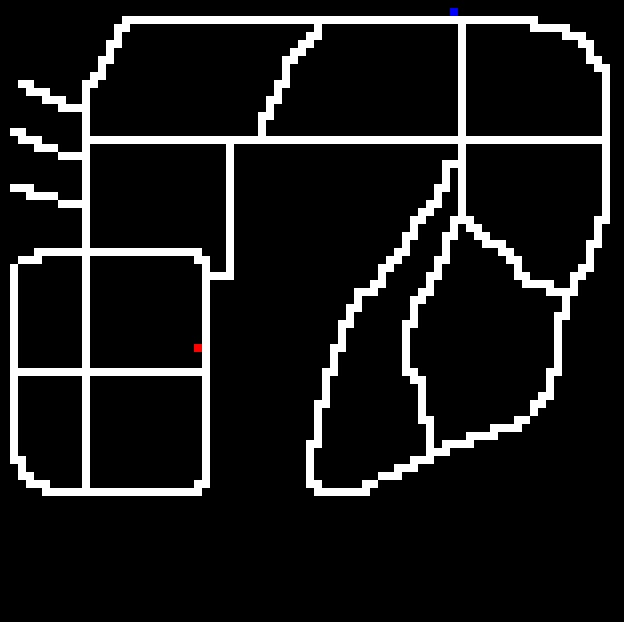
\includegraphics[scale=0.6]{images/AStarProblem.jpg}
\caption{Teszt bemenet}
\label{fig:model1problem}
\end{figure}

A megoldást felhasználva a következő képet adja válaszul.

\begin{figure}[h!]
\centering
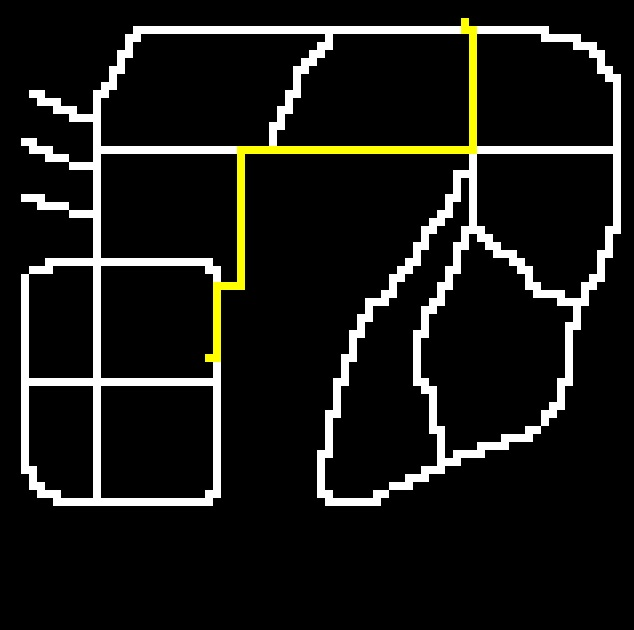
\includegraphics[scale=0.6]{images/AStarResult.jpg}
\caption{Teszt kimenet}
\label{fig:model1result}
\end{figure}

A kép kíválóan szemlélteti, hogy a optimális utat adott eredményül, ezáltal az algoritmus felhasználható az adott feladathoz.


\Chapter{Egy étterem, egy futár, több kiszállítás esete}


\Section{
A probléma megfogalmazása
}

Egy étterem, egy futár és több kiszállításnál az adott helyzet egészen visszavezethető a klasszikus utazó ügynök problémához.
A futár elindul az étteremből, érinteni kell az összes kiszállítási pontot, valamint vissza kell érkeznie az étterembe, mindezt úgy, hogy a lehető legkisebb utat tegye meg.

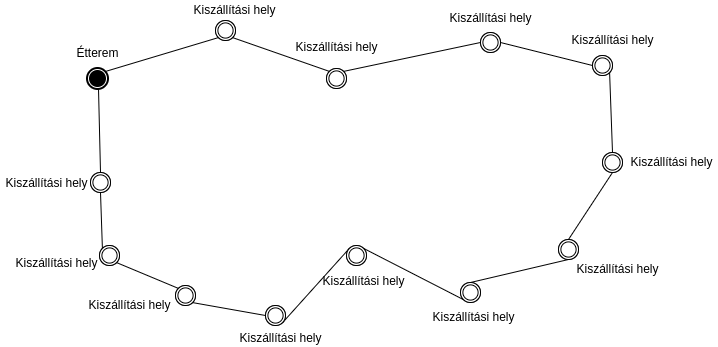
\includegraphics[scale=0.5]{images/Simpletsp.png}

\Section{
A probléma megoldása
}

Gibbs faktor \\

A klasszikus utazó ügynök probléma matematikai megfogalmazása kiszállítási kritériumokra levetítve\\

Az egy ügynökös utazó ügynök probléma esetén jelölje V a csúcsok (pontok) halmazát, xi,j azt, hogy az i. pontból megy-e közvetlenül út a j. pontba. Az xi,j 1, ha útvonal köti össze a két pontot, különben 0:


\includegraphics[scale=0.5]{images/1tsp.png}

A dij jelöli az i. és a j. pont távolságát, n pedig a pontok számát. A célfüggvény az alábbi:

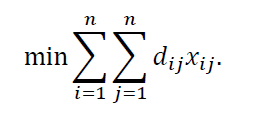
\includegraphics[scale=0.5]{images/2tsp.png}

A célfüggvénnyel magát a megtett távolságot szeretnénk optimalizálni. A pontba csak egy él fut be, tehát

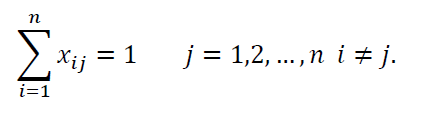
\includegraphics[scale=0.5]{images/3tsp.png}

Valamint, minden pontba csakis egy él távozik, ezek szerint

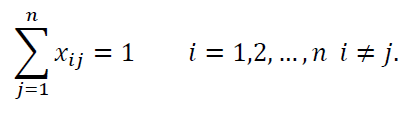
\includegraphics[scale=0.5]{images/4tsp.png}

A sorrendiség a következő feltétel alapján érényesül

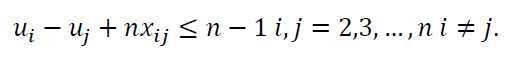
\includegraphics[scale=0.5]{images/5tsp.png}

Itt ui az i. pont, uj a j. pont látogatási indexe, ahol az i. pontot hamarabb keresi fel az futár mint a j.-ot

\Section{A megoldás implementálása}

Összes lehetséges út:
\[
\dfrac{(n-1)!}{2}
\]
Ezek közül kell választanunk, ez ugyanis a Hamilton-körök száma az n pontú teljes gráfban.

A képlet csak $n > 2$ esetén működik.

Ezen importok szükségesek a szimuláció futtatásához

\begin{python}
from scipy.spatial import distance_matrix
\end{python}

A cél az, hogy listát készítsünk a pontokról, amelyek mindegyike két koordinátát tartalmaz $(x, y)$, amelyek 0 és 100 közötti véletlen egész számokként kerülnek kiválasztásra. Jelen esetben 10 ilyen pont lesz.

\begin{python}
points = [random.sample(range(100), 2) for x in range(10)]
\end{python}

A pontok közötti távolságok kimutatását így oldottam meg.

\begin{python}
data = Points
points = ['1', '2', '3', '4', '5', '6', '7', '8', '9', '10']
df = pd.DataFrame(data, columns=['xcord', 'ycord'], index=points)
pd.DataFrame(
	distance_matrix(
		df.values, 
		df.values
	), 
	index=df.index,
	columns=df.index
)
\end{python}

Ezt a kimenetett adta válaszul.

\begin{figure}[h!]
\centering
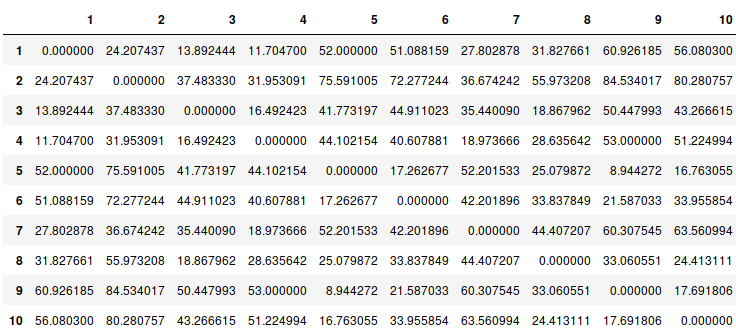
\includegraphics[width=\textwidth]{images/table.png}
\caption{Kimenet}
\label{fig:kimenet}
\end{figure}

Inicializáljuk a pointCount értékét 10-re, ennyi helyre kell a futárnak eljutnia.

\begin{python}
pointCount = 10
\end{python}

A travel egy adott számból álló lista (jelen esetben 10 számból áll), amely a pontok meglátogatására utal. Feltételezzük, hogy zárt hurokra van szükség, így az utolsó pont autómatikusan csatlakozik az elsőhöz.


\begin{python}
travel = random.sample(range(pointCount), pointCount);}
\end{python}

Elindítunk egy ciklust az adott értékekkel


\begin{python}
for tlp in numpy.logspace(0, 5, num = 100000)[::-1]:
\end{python}


Két pont véletlenszerű cseréjével új új utat képzünk. Úgy valósítom meg, hogy választok két számot az i-t és a j-t. Összeállítom a newTravel-t a régi travel másolásával az i indexig, majd összefűzöm a j-edik travelel-t és egészen folytatom addig, amíg a j nem éri el az i-edik pontot, majd befejezem a travel többi részét.


\begin{python}
[i, j] = sorted(random.sample(range(pointCount), 2));
newTravel = travel[:i] + 
			travel[j:j + 1] + 
			travel[i + 1:j] + 
			travel[i:i + 1] + 
			travel[j + 1:]
\end{python}


Ha az if értéke igaz akkor a travel megkapja a newTravel értékét, az előzöekben említett csere miatt ez már változott. Az elképzelés az, hogy minimalizálni szeretnénk a pontok közti távolságok költségének összegét. Ehhez a Gibb-s faktor-t használtam fel, aminek lényege, az új állapotba való átmenet valószínűsége. Csak az i-edik és j-edik pontok közötti távolságokat szükséges összegezni, mivel a többi távolság ugyanaz mint a travel-ben mint a newTravel-ben egyaránt. Ha a faktor > 1 akkor az új költség alacsonyabb, travel megkapja a newTravel értékét.


\begin{python}
traveld = sum([
	math.sqrt(
		sum([(
			(
			  (points[travel[(k + 1) % pointCount]][d]) - 
			  (points[travel[k % pointCount]][d])
			) **  2
		) for d in [0, 1]])
	) for k in [j, j - 1, i, i - 1]
])
newTraveld = sum([
	math.sqrt(
		sum([(
			(
			  (points[newTravel[(k + 1) % pointCount]][d]) - 
			  (points[newTravel[k % pointCount]][d])) 
			** 2
		) for d in [0, 1]])
	) for k in [j, j - 1, i, i - 1]
])
    if math.exp((traveld - newTraveld) / tlp) > random.random():
        travel = copy.copy(newTravel);
\end{python}        


Az algoritmus végeztével már csak meg kell jeleníteni a kívánt pontokat, ez kirajzol egy gráfot, amely optimális utat ad. Ehhez a pyplot libary-t használtam


\begin{python}
plt.plot(
	[points[
		travel[i % pointCount]][0] for i in range(pointCount + 1)
	], 
	[points[
		travel[i % pointCount]][1] for i in range(pointCount + 1)
	], 
	'xb-'
)
plt.show()
\end{python}

Kapcsolódó problémák

Adott teljes élsúlyozott gráf esetén keressük a legkisebb összsúllyal rendelkező Hamilton-kört. Megmutatható, hogy a kiindulási városba való visszatérés megkövetelése nem nehezít a probléma számítási nehézségén, tehát minimális súlyú Hamilton-út keresése egy adott pontból is NP-teljes.
A probléma egy másik változata, amikor nem a legkisebb súlyú Hamilton-kört keressük, hanem azt, amelyikben a „legnehezebb” él súlya a lehető legkisebb. A logisztikai problémákon túl nagy gyakorlati jelentőséggel bír például a nyomtatott áramkörök gyártása során fúrórobotok ideális mozgásának megtervezésében.

\Section{A megoldás tesztelése}

5 város esetén
Összehasonlítások száma: 74 434
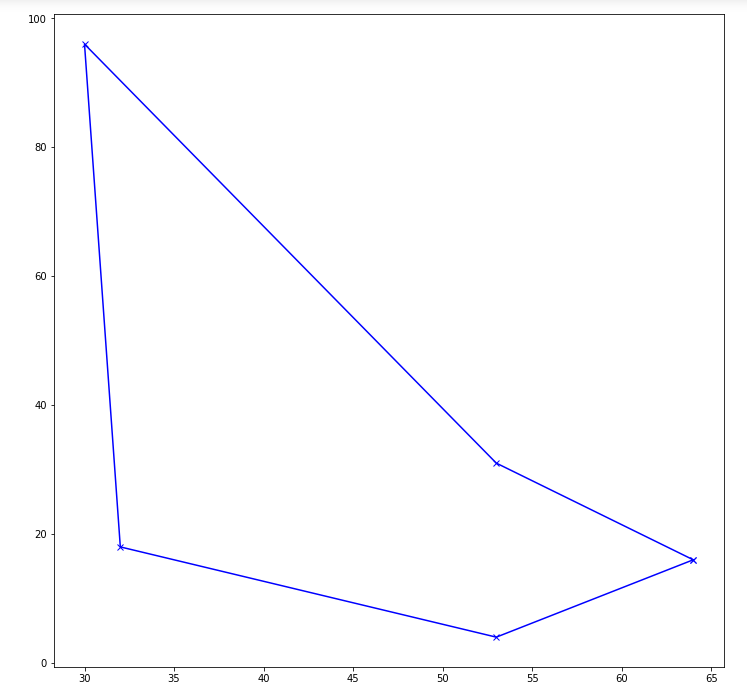
\includegraphics[scale=0.4]{images/5.png}

10 város esetén
Összehasonlítások száma: 68 594
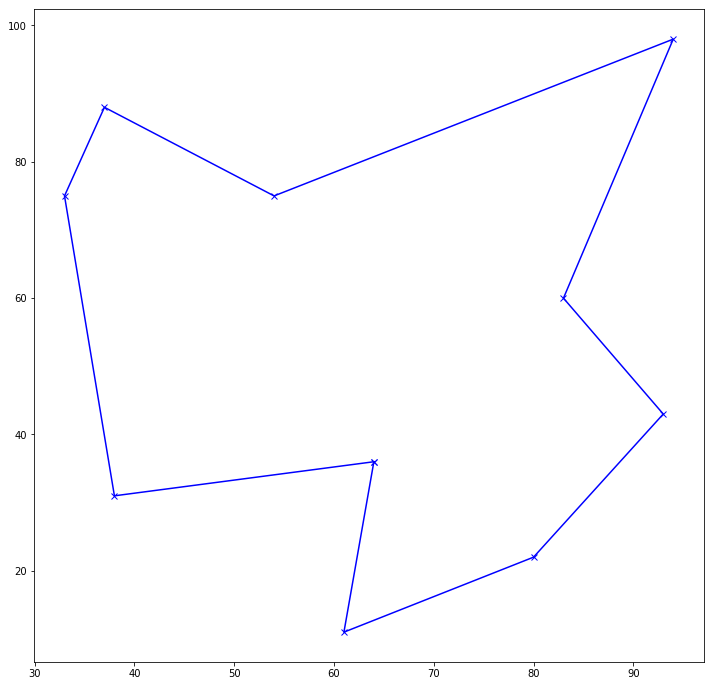
\includegraphics[scale=0.4]{images/10.png}

15 város esetén
Összehasonlítások száma: 66 672
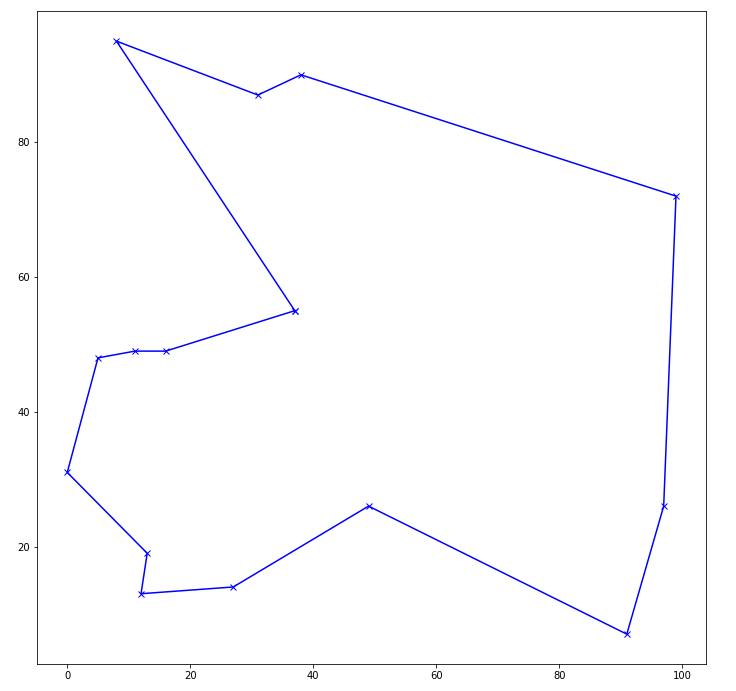
\includegraphics[scale=0.4]{images/15.png}

20 város esetén
Összehasonlítások száma: 65 265
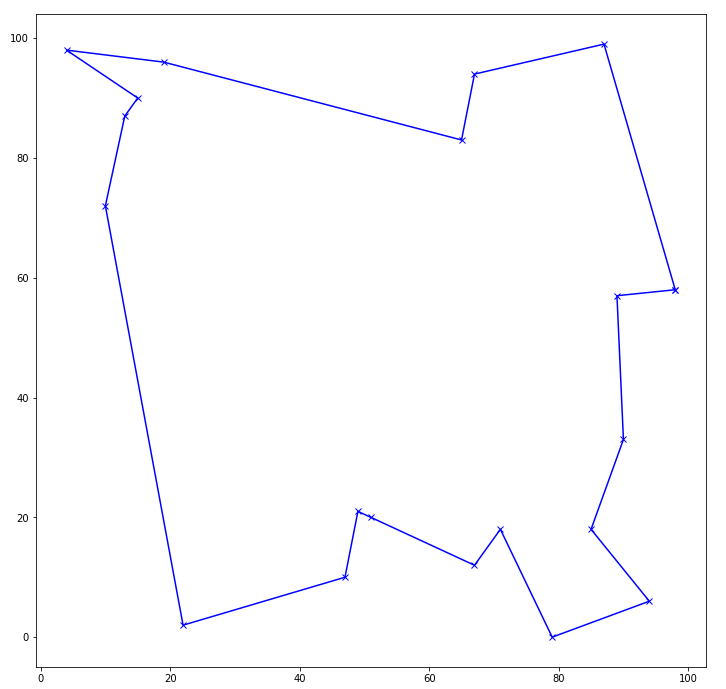
\includegraphics[scale=0.4]{images/20.png}

25 város esetén
Összehasonlítások száma: 67 865
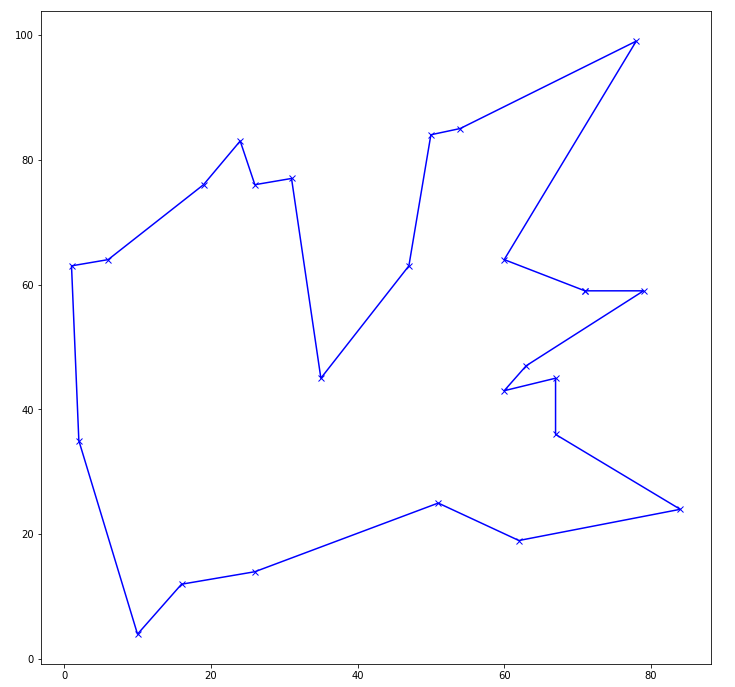
\includegraphics[scale=0.4]{images/25.png}

30 város esetén
Összehasonlítások száma: 65 324
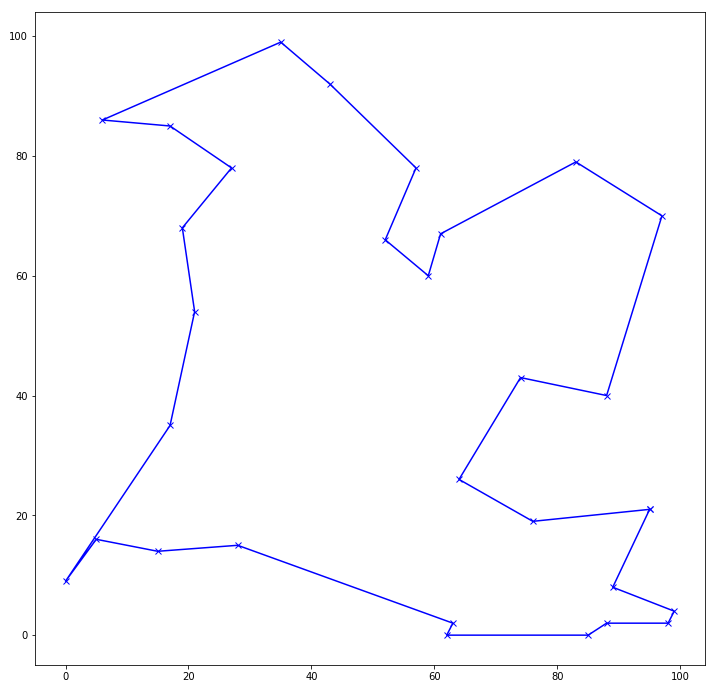
\includegraphics[scale=0.4]{images/30.png}

35 város esetén
Összehasonlítások száma: 67 230
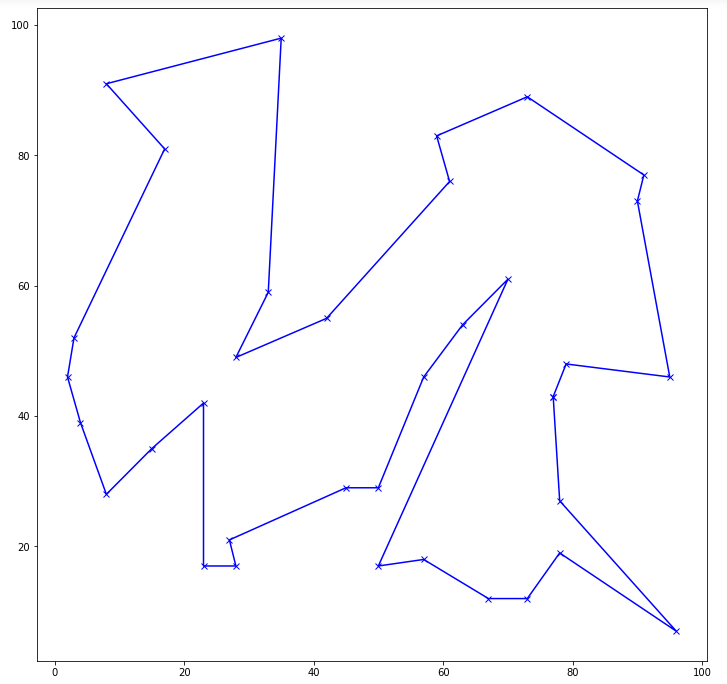
\includegraphics[scale=0.4]{images/35.png}

40 város esetén
Összehasonlítások száma: 66 008
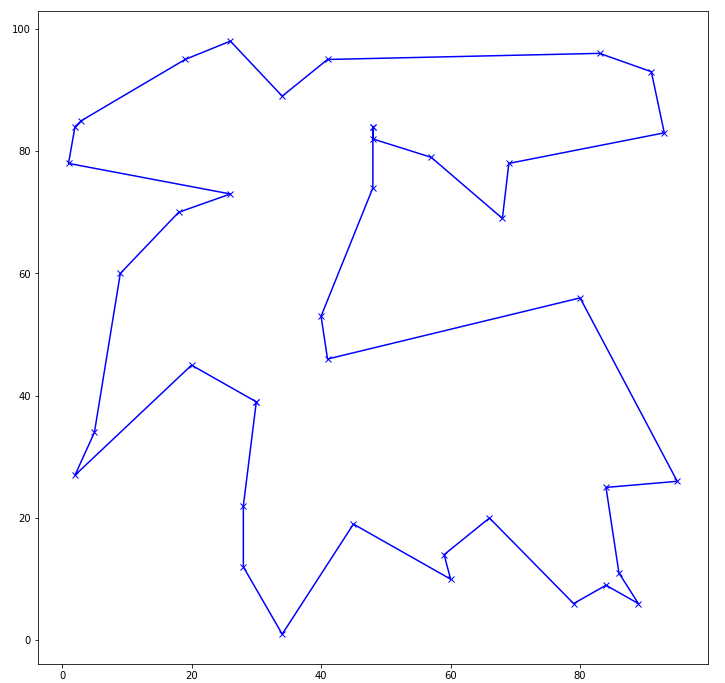
\includegraphics[scale=0.4]{images/40.png}


Több lefuttatott teszt után is megfgyelhető, hogy az összehasonlítások száma 65 ezer és 75 ezer között mozog. Egytől egyig az optimális utat adták.

A következő gráfok megmutatják a kívánt utat vároksok száma szerint. Mivel véletlenszerű számok összehasonlításán alapszik az algoritmus ezáltal az összehasonlítások száma igen magas, viszont stagnál bizonyos értékek között.

\Chapter{Több étterem, egy futár, több kiszállítás esete}

\Section{A probléma megfoglmazása}

Több étterem esetén meg kell határozni néhány feltételt. Jelen helyzetben a futár elindul az egyik étteremből, kiszállít mindent, majd egy másik étterembe érkezik ezt követően, és annak a rendeléseit is kiszállítja. Időben is meg kell szabni néhány határt, miszerint az első étteremből való indulás pillanatáig beérkezett rendeléseket szállítja csak ki az összes étteremből. Miután sikeresen kivitte az összes rendelést visszatér a kezdő étterembe és kezdődik előlről a folyamat. Maga a folyamat egy önmagát ismételő klasszikus utazó ügynök probléma, annyi eltéréssel, hogy nem ugyan abba az étterembe kell érkeznie ahonnan indult, hanem a hozzá legközelebb esőbe amelyikbe még nem járt az adott ciklusban. A probléma szemléltetése \aref{fig:model3}. ábrán látható \cite{Diagrams.net}.

\begin{figure}[h!]
\centering
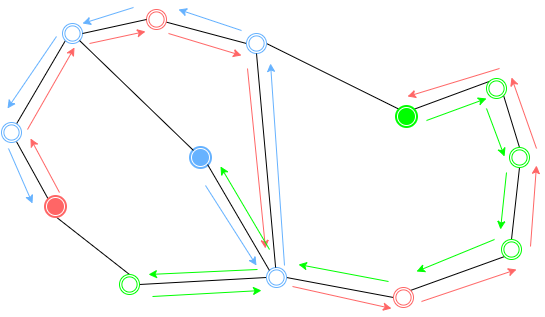
\includegraphics[scale=0.6]{images/Circulartsp.png}
\caption{Több étterem, egy futár, több kiszállítás modellje}
\label{fig:model3}
\end{figure}


\Section{A probléma megoldása}

Maga a probléma egy már megoldott helyzetre vezethető vissza. Az egy étterem, egy futár, több kiszállítás eseténél mindig ugyanabba az egy étterembe kellett visszatérnie a futárnak. Az ott alkalmazott módszerek érvényesek erre az esetre is, annyi eltéréssel, hogy ha kiszállította egy étterem rendeléseit az utolsó megállóhelye a folyamatban a következő étterem (nem az amiből indult). A folyamat következő lépése pedig innen indul, a futár kiszállítja az összes rendelést és egy harmadik étterembe érkezik utolsóképp. Ez mindaddig tart, amíg a futár meg nem látogatja az összes éttermet és vissza nem tér a kezdő, kiinduló étterembe. 

\Section{A megoldás implementálása}

Az előző megoldást felhasználva, pár változtatást el kellett végezni, hogy helyesen működjön erre az esetre.

Be kellett vezetni egy összegzést ami az éttermek számát határozza meg \cite{Python}.
\begin{python}
restaurantCount = 4
\end{python}
Ezt követően feltöltöttem egy listát véletlenszerűen generált $x$ és $y$ koordinátákkal. Maga a lista hossza az előbb meghatározott \texttt{restaurantCount}-al egyenlő.
\begin{python}
restaurants = [random.sample(range(100),2)
               for x in range(restaurantCount)] 
\end{python}
Szükségszerű volt bevezetni egy külső ciklust, ami az éttermek számáig megy. Ezáltal nyerhetőek vissza az adott étterem koordinátái.
\begin{python}
for l in range(len(restaurants)):
\end{python}
A cikluson belül a pontok számát csökkentenünk kellett egyel, valamint az első helyre hozzáadni a \texttt{restaurants} adott \texttt{l} elemét. Ezáltal meg van oldva, hogy a ciklus mindig az éttermektől induljon.

\begin{python}
travel = [random.sample(range(100), 2) for x in range(pointCount - 1)]
travel.insert(0, restaurants[l])
\end{python}

Meg kell még oldani, hogy a ciklus utolsó eleme a következő étterem koordinátája legyen. Figyelembe kellett venni azt is, hogy az utolsó étterem utolsó pontja az első étterem koordinátáival kell, hogy megegyezzenek. Szükségessé vált a kör megszakítása is a gráfban. 
Ezek a következőképpen néznek ki. 
\begin{python}
helperX = travel[i % pointCount]][0] for i in range(pointCount)
helperY = travel[i % pointCount]][1] for i in range(pointCount)

if l < (len(restaurants) - 1):
	helperX.append(restaurants[l+1][0])
	helperY.append(restaurants[l+1][1])
else:
	helperX.append(restaurants[0][0])
	helperX.append(restaurants[0][1])
\end{python}

\Section{A megoldás tesztelése}

A módszer vizsgálatához 4 éttermet és 36 kiszállítási helyet vettem számításba.
Az elkészített program által visszaadott útvonalak \aref{fig:tspMR1}., \ref{fig:tspMR2}., \ref{fig:tspMR3}.  és \ref{fig:tspMR4}. ábrán láthatók.
Jól megfigyelhető, hogy az utolsó étterem utolsó pontja visszatér az első étterem koordinátáihoz a (71, 42) pontba.

\begin{figure}[h!]
\centering
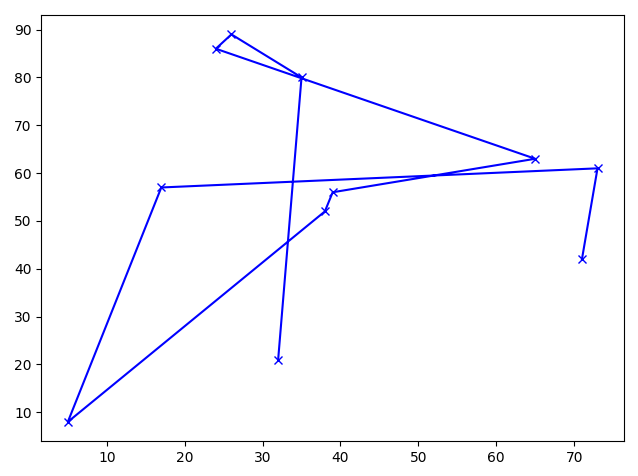
\includegraphics[scale=0.8]{images/tsp1MR.png}
\caption{Első étterem poziciója: (71, 42)}
\label{fig:tspMR1}
\end{figure}

\begin{figure}[h!]
\centering
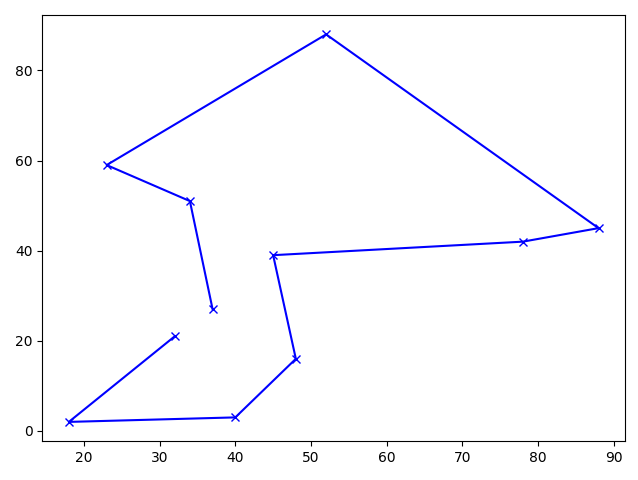
\includegraphics[scale=0.8]{images/tsp2MR.png}
\caption{Második étterem poziciója: (32, 21)}
\label{fig:tspMR2}
\end{figure}

\begin{figure}[h!]
\centering
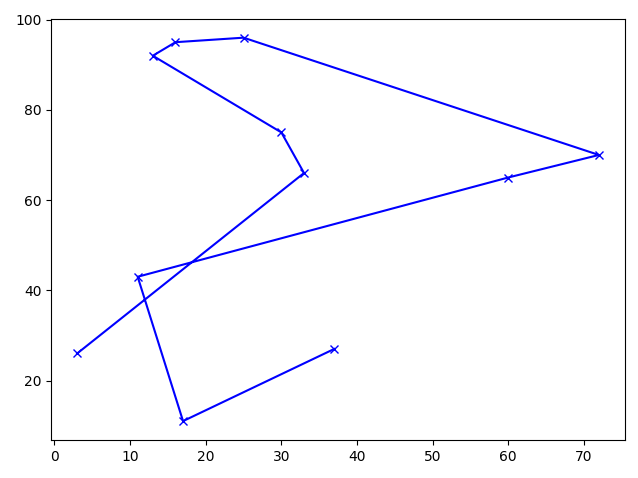
\includegraphics[scale=0.8]{images/tsp3MR.png}
\caption{Harmadik étterem poziciója: (37, 27)}
\label{fig:tspMR3}
\end{figure}

\begin{figure}[h!]
\centering
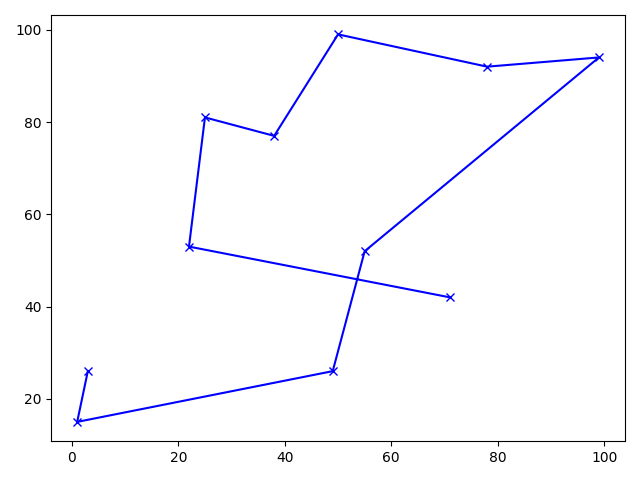
\includegraphics[scale=0.8]{images/tsp4MR.png}
\caption{Negyedik étterem poziciója: (3, 26)}
\label{fig:tspMR4}
\end{figure}
\Chapter{Egy étterem, több futár, több kiszállítás esete}

\Section{A probléma megfoglmazása}

Jelen eset reprezentálja az egy lerakatos több ügynökös utazó ügynök problémát. Feltételek meghatározásánál nélkülözhetetlen szempont, hogy határokat szabjunk az egyes futároknak, hogy ki milyen területre szállít ki. Ennek meghatározásánál fontos a kiszállítási címek közti táv figyelembe vétele. Ezek meghatározása után maga a probléma leegyszerűsíthető egy klasszikus utazó ügynök problémára.

\begin{figure}[h!]
\centering
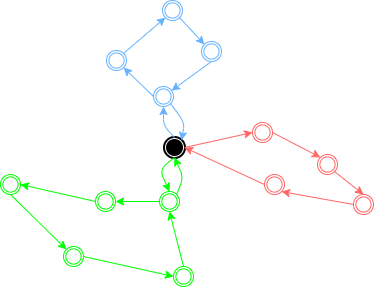
\includegraphics[scale=0.7]{images/Onedepotmtsp.png}
\caption{Egy étterem, több futár, több kiszállítás modellje}
\label{fig:model4}
\end{figure}

\Section{A probléma megoldása}

A több ügynökös, egy lerakatos utazó ügynök probléma modellje kiszállítási helyzetekre szabva\\

A több ügynökös, egy lerakatos utazó ügynök probléma esetén legyen V a csúcsok halmaza, $x_{i,j}$ az, hogy megy-e az $i.$ pontból út a $j.$ pontba közvetlenül, $d_{i.j}$ az $i.$ és $j.$ pont távolsága. Legyen $m$ az ügynökök száma és ezáltal a kapott célfüggvény:

\begin{figure}[h!]
\centering
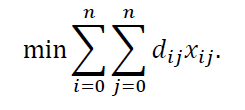
\includegraphics[scale=0.5]{images/mtsp1.png}
\end{figure}

Minden pontba csakis egy út indul, kivétel ez alól a 0. pont ami maga az étterem:

\begin{figure}[h!]
\centering
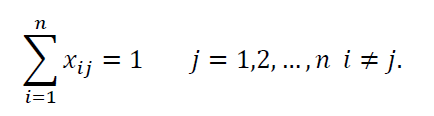
\includegraphics[scale=0.5]{images/mtsp2.png}
\end{figure}

Minden pontból csak egy út érkezik, kivétel ez alól a 0. pont ami maga az étterem:

\begin{figure}[h!]
\centering
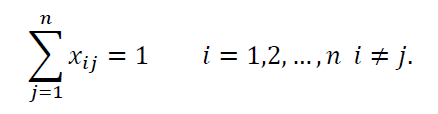
\includegraphics[scale=0.5]{images/mtsp3.png}
\end{figure}

Az étteremre való feltétel:

\begin{figure}[h!]
\centering
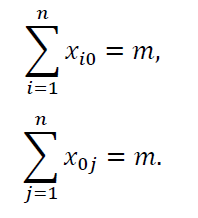
\includegraphics[scale=0.5]{images/mtsp4.png}
\end{figure}

MTSP esetén a kövezkező megszorítások szükségessége elengedhetetlen a helyes sorrendmátrix beteljesüléséhez:

\begin{figure}[h!]
\centering

\includegraphics[scale=0.5]{images/mtsp5.png}
\end{figure}

A definícióban $S$ a pontok egy részhalmaza, $r(S)$ pedig az, hogy ezt a részthalmazt minimum hány futárnak kell látogatnia. A definíció szumma része megmutatja, hogy minimum hány út megy be a vizsgált pontba. Az éttermet figyelmen kívűl hagyjuk m darab út hagyja el és m darab út megy ki belőle. Ezáltal a fenti egyenlőtlenség nem a futárok tényleges számát adná vissza. 

Magát a problémát genetikus algoritmussal oldottam meg.\\

Genetikus algoritmus \\

A genetikus algoritmust számítógépes szimulációkkal reprezentálják. A keresési teret populációs egyedek alkotják. Ezen egyedeket lehet keresztezni (más szóval rekombinálni) és mutálni is, ezáltal új egyedek kreálhatóak. Fitnesz függvénynek nevezzük a keresési téren értelmezett célfüggvényt. Az alfgoritmus működése során új egyedeket képes létrehozni a rekombinációs és mutációs operátorokkal, valamint kiszűri a rosszabb fitnesz függvény értékkel rendelkező egyedeket, majd ezt követően kiszedi azokat a populációból.

Folyamata: \\

1. Inicializáció:  Az induló populációt legkönnyebben véletlenszerű számokkal tudjuk létrehozni. Maga a populáció mérete erősen függ a problémától. A keresési téren az egyedek általában egyenletesen oszlanak el, viszont számos esetben több egyedet generál a feltételezhető optimum közelében. \\

2. Kiválasztás: Az összes eredményes generációban szelekcióra kerül az aktuális populáció egy része szaporodásra. A kiválasztás rendszerint fitnesz alapján történik, ahol a fitnesz függvény szerinti legfitebb egyedek valószínűbben kerülnek szelekcióra. Számos metódus az összes egyed fitneszét figyelembe veszi és ezek alapján keresi a legjobbat. Akadnak olyan metódusok is amik csak néhány véletlenszerűen kiválasztott példányt vizsgálnak. A példány minőségének mérésére használják a fitnesz függvényt. Ezen függvény bonyolultsága minden esetben a problémától függ. \\

3. Szaporítás: Egyoperandusú mutációval valamint kétoperandusú keresztezési műveletek által lehetséges a példányokból újabb példányokat kreálni. Ezen operátorokat véletlenszerűen használják. \\

4. Leállás: A genetikus algoritmus addig fut amíg be nem teljesül a leállási feltétel.\\

Előnye: Kedvező eredménnyel használható majdnem minden problémára. Folytonos, illetve diszkrét problémáknál úgyszintén alkalmazható. A folyamatok könnyen páhuzamosíthatóak általa.

Hátránya: A megfelelő operátor kiválasztása nehéz. Paraméterezése és a leállási feltétel meghatározása sok időt igényel, valamint nem garantált a globális optimum elérése.

Elitizmus: Ebben az esetben a jelenlegi populáció legjobb egyedét mindig, módosítás nélkül visszük tovább az új populációba.

\Section{A megoldás implementálása}

\subsection{
Dustbin
}

\begin{figure}[!htb]
\centering
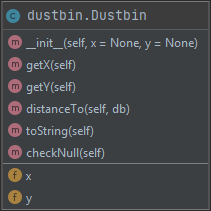
\includegraphics[scale=0.7]{images/dustbin.png}
\caption{Dustbin osztálydiagram}
\label{fig:dustbin}
\end{figure}

Inicializáló metóduson kívűl található benne még olyan folyamat ami felel, az x és y értékek feldolgozásával. Ezen felül az euklidészi távolság számítás is itt foglal helyet. Utolsó sorban pedig egy formázó metódus ami a szöveget helyesen formázottan adja vissza.

\subsection{
Galogical
}

Az eljárás lényegi, logikai része itt valósul meg.

\begin{figure}[!htb]
\centering
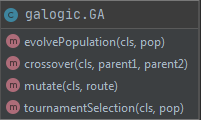
\includegraphics[scale=0.8]{images/galogic.png}
\caption{Galogical osztálydiagram}
\label{fig:galogical}
\end{figure}

A populáció fejlesztésére használt metódus. Tartalmaz egy ellenőrzést, hogy kívánunk-e elitizmussal élni a futás alatt vagy sem. Ezenfelül a keresztezés és mutáció operátorokat meghívó programkódok is itt foglalnak helyet.

\begin{python}
@classmethod
def evolvePopulation(cls, pop):

    newPopulation = Population(pop.populationSize, False)

    elitismOffset = 0
    if elitism:
        newPopulation.saveRoute(0, pop.getFittest())
        elitismOffset = 1

    for i in range(elitismOffset, newPopulation.populationSize):
        parent1 = cls.tournamentSelection(pop)
        parent2 = cls.tournamentSelection(pop)
        child = cls.crossover(parent1, parent2)
        newPopulation.saveRoute(i, child)

    for i in range(elitismOffset, newPopulation.populationSize):
        cls.mutate(newPopulation.getRoute(i))

    return newPopulation
\end{python}
A keresztezési operátor implementációját a következőképpen kódoltam.

\begin{python}
@classmethod
def crossover (cls, parent1, parent2):
    child = Route()
    child.base.append(Dustbin(-1, -1))
    startPos = 0
    endPos = 0
    while (startPos >= endPos):
        startPos = random.randint(1, numNodes-1)
        endPos = random.randint(1, numNodes-1)

    parent1.base = [parent1.route[0][0]]
    parent2.base = [parent2.route[0][0]]

    for i in range(numDeliverer):
        for j in range(1, parent1.routeLengths[i]):
            parent1.base.append(parent1.route[i][j])

    for i in range(numDeliverer):
        for j in range(1, parent2.routeLengths[i]):
            parent2.base.append(parent2.route[i][j])

    for i in range(1, numNodes):
        if i > startPos and i < endPos:
            child.base[i] = parent1.base[i]

    for i in range(numNodes):
        if not(child.containsDustbin(parent2.base[i])):
            for i1 in range(numNodes):
                if child.base[i1].checkNull():
                    child.base[i1] =  parent2.base[i]
                    break

    k=0
    child.base.pop(0)
    for i in range(numDeliverer):
        child.route[i].append(RouteManager.getDustbin(0))
        for j in range(child.routeLengths[i]-1):
            child.route[i].append(child.base[k])
            k+=1
    return child
\end{python}
A mutáció operátor kódja az alábbi.

\begin{python}
@classmethod
def mutate (cls, route):
    index1 = 0
    index2 = 0
    while index1 == index2:
        index1 = random.randint(0, numDeliverer - 1)
        index2 = random.randint(0, numDeliverer - 1)

    route1startPos = 0
    route1lastPos = 0
    while route1startPos >= route1lastPos or route1startPos == 1:
        route1startPos = random.randint(1, route.routeLengths[index1] - 1)
        route1lastPos = random.randint(1, route.routeLengths[index1] - 1)

    route2startPos = 0
    route2lastPos = 0
    while route2startPos >= route2lastPos or route2startPos == 1:
        route2startPos = random.randint(1, route.routeLengths[index2] - 1)
        route2lastPos= random.randint(1, route.routeLengths[index2] - 1)

    swap1 = []
    swap2 = [] 

    if random.randrange(1) < mutationRate:
        for i in range(route1startPos, route1lastPos + 1):
            swap1.append(route.route[index1].pop(route1startPos))

        for i in range(route2startPos, route2lastPos + 1):
            swap2.append(route.route[index2].pop(route2startPos))

        del1 = (route1lastPos - route1startPos + 1)
        del2 = (route2lastPos - route2startPos + 1)

        route.route[index1][route1startPos:route1startPos] = swap2
        route.route[index2][route2startPos:route2startPos] = swap1

        route.routeLengths[index1] = len(route.route[index1])
        route.routeLengths[index2] = len(route.route[index2])
\end{python}

A tournamentSelection metódus kiválasztja a legfitebb kromószómahalmazt.

\begin{python}
@classmethod
def tournamentSelection (cls, pop):
    tournament = Population(tournamentSize, False)

    for i in range(tournamentSize):
        randomInt = random.randint(0, pop.populationSize-1)
        tournament.saveRoute(i, pop.getRoute(randomInt))

    fittest = tournament.getFittest()
    return fittest
\end{python}

\subsection{
Globals
}

Az inicializáló adatokat foglalja magában, ezen kívűl még két metódust is tartalmaz.

Az inicializáló adatokat három részre lehet osztani.

1. A koordináták tartományát lehet vele manipulálni.

\begin{python}
xMax = 100
yMax = 100
seedValue = 1
numNodes = 40
numGenerations = 20
\end{python}

2. A populációra vonatkozó adatok itt módosíthatóak.

\begin{python}
populationSize = 20
mutationRate = 0.02
tournamentSize = 1
elitism = True
\end{python}

3. Ezen részben lehet megadni a futárok számát is.

\begin{python}
numDeliverer = 2
\end{python}

A két metódus pedig random adatok generálására szolgál.

\subsection{
Main
}

Maga a futtatható metódus. Ebben értékelődik ki az optimális útvonal valamint egy diagram ami y tengelyén látható a fittnesz függvény érték (távolság), x tengelyén pedig a generációk száma.

\subsection{
Population
}

\begin{figure}[!htb]
\centering
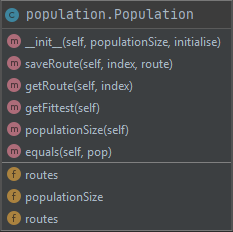
\includegraphics[scale=0.8]{images/population.png}
\caption{Population osztálydiagram}
\label{fig:population}
\end{figure}

Az egyedeken végzett műveletekhez szükséges oszály. Tartalmaz egy inicializáló metódust, ezen felül itt kapott helyet az út mentése, kiolvasása is. A legfitebb érték meghatározásán kívűl a populációk összehasonlításával is foglalkozik az oszály. 

\subsection{
Route
}

\begin{figure}[!htb]
\centering
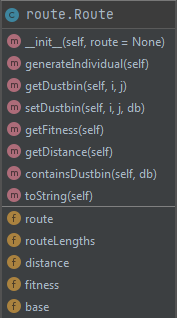
\includegraphics[scale=0.8]{images/route.png}
\caption{Route osztálydiagram}
\label{fig:route}
\end{figure}

Az optimális út kiszámításához használt osztály. Az alap inicializáláson kívűl jelen vannak még a helyes út kiszámításához használatos metódosok. Végezetül egy szövegformázó metódus is itt kapott helyet.
\\\
\\\
\\\
\\\

\subsection{
Routemanager
}

\begin{figure}[!htb]
\centering
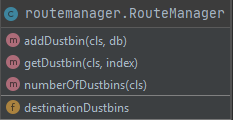
\includegraphics[scale=0.8]{images/routemanager.png}
\caption{Routemanager osztálydiagram}
\label{fig:routeManager}
\end{figure}

Az oszály egyedeket kezel, három osztálymetódusból áll amik az optimális út eléréséhez nélkülözhetetlenek.

\\\
\\\
\\\
\\\
\\\
\\\

\Section{A megoldás tesztelése}

\subsection{
Elitizmus nélkül
}

A kiszállítási helyek száma: 40\\
Generációk száma: 40\\
Populáció nagysága: 20\\
Elitizmus: Hamis\\
Futárok száma: 3\\

\begin{figure}[!htb]
\centering
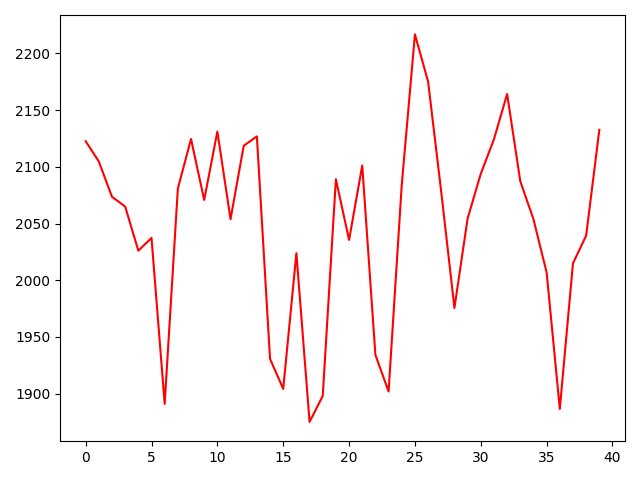
\includegraphics[scale=0.7]{images/MTSPMultiDepo1.png}
\caption{Fitnessz értékek generiónként elitizmus nélkül}
\label{fig:MTSPMultiDepo1}
\end{figure}

\begin{figure}[!htb]
\centering
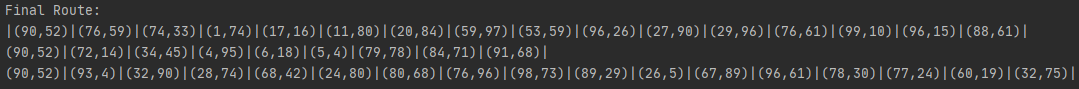
\includegraphics[width=\textwidth]{images/MTSPMultiDepo1Route.png}
\caption{Futárok útjai elitizmus nélkül}
\label{fig:MTSPMultiDepo1Route}
\end{figure}

\subsection{
Elitizmussal
}

A kiszállítási helyek száma: 40\\
Generációk száma: 40\\
Populáció nagysága: 20\\
Elitizmus: Igaz\\
Futárok száma: 3\\

\begin{figure}[!htb]
\centering
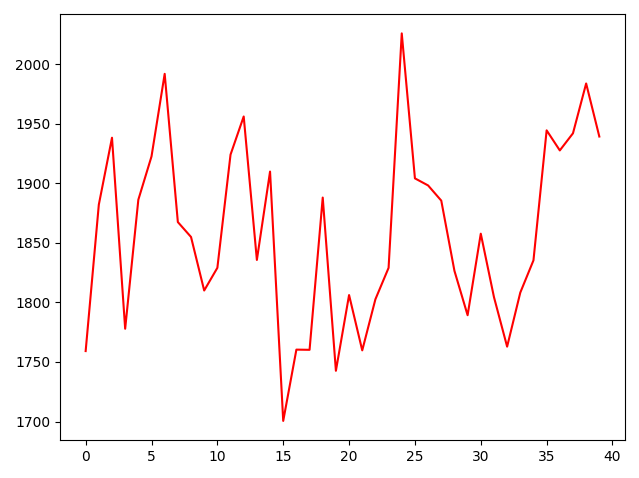
\includegraphics[scale=0.7]{images/MTSPMultiDepo2.png}
\caption{Fitnessz értékek generiónként elitizmussal}
\label{fig:MTSPMultiDepo2}
\end{figure}

\begin{figure}[!htb]
\centering
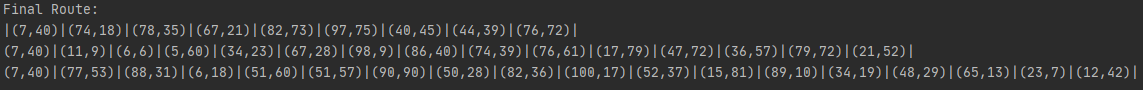
\includegraphics[width=\textwidth]{images/MTSPMultiDepo2Route.png}
\caption{Futárok útjai elitizmussal}
\label{fig:MTSPMultiDepo2Route}
\end{figure}

\Chapter{Több étterem, több futár, több kiszállítás esete}

\Section{A probléma megfoglmazása}

Ez az eset tisztán leírja a több lerakatos több ügynökös utazó ügynök problémát. Jelen esetben tisztázni kell, hogy a futárok különböző éttermekből indulnak ki. Próbálnak keresni egy olyan utat, aminek költésége viszonylag kicsi, tehát a közeli helyekhez tartozó csomagot veszik csak fel és szállítják ki. Ezt követően a legközelebbi kiszállítási helyet vizsgálják. Figyelembe veszik a szükségesen meglátogatni kívánt étterem körüli kiszállítási helyket, és ez alapján választják meg az útjukat. Amennyiben ez az út túl költésges lenne, akkor próbálnak keresni egy másikat célt, aminél kevesebb út befektetésével több címet tud meglátogatni. Mindezek mellett, hogy a folyamatban ne legyen többszöri meglátogatás, a futároknak tudniuk kell, hogy ki hol járt már, hol történt meg a kiszállítás sikeresen.
A model egy szemléltetését láthatjuk \aref{fig:model5}. ábrán.

\begin{figure}[h!]
\centering
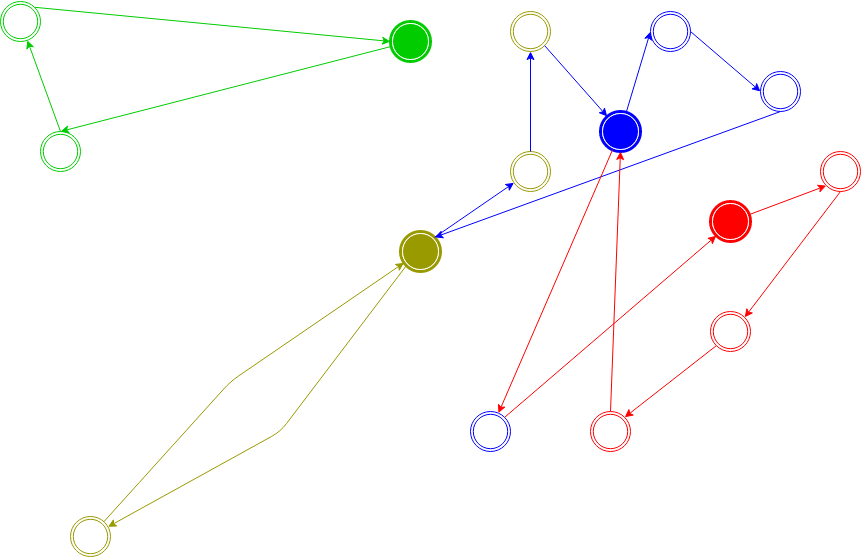
\includegraphics[scale=0.45]{images/model5.png}
\caption{Több étterem, több futár, több kiszállítás modellje}
\label{fig:model5}
\end{figure}

\Section{A probléma egy lehetséges megoldása}

Első lépésként véletlenszerű pontokat kell generálnunk. Ezek jelképezik majd a kiszállítási helyeket. Ezt követően meg kell határoznunk az éttermek számát, majd legenerálni őket véletlenszerű helyekre. Később meg kell határoznunk egy átlagos távolságot, ami a különböző kiszállítási pontok közötti távolságok átlagának felel meg. Nyilván kell tartanunk, hogy ki melyik étteremből rendelt, hogy ezáltal mindenképp az éttermet kelljen előbb meglátogatni, ha a csomag még egyik futárnál sincs. Tekintettel kell lenni a futárok aktuális helyezetére, hiszen ha elfogyott a csomagja, keresni fogja a legközelebbi pontot ahova viheti majd a szállítmányt. Nélkülözhetetlen meghatározni a futárok útjait. Ehhez szükséges az előzőekben meghatározott átlag szakasz. A folyamat felépítésére tekintettel szükséges egy fő ciklus, mely a futárok számáig megy. Ezen belül megy egy másik ami a futár útjain megy végig. Ezen megoldás gyakorlati alkalmazása esetén lehetséges optimalizálni a kiszállításokat egy ilyen összetett modell esetén is.

Ezen optimalizálási feladat részletesebb vizsgálata még további kutatások tárgyát képezi.

\Chapter{Összefoglalás}

A dolgozatom témája az éttermi rendelések optimalizációja és szimulációja, amely segít meghatározni, az optimálus útvonalat a futároknak kiszállítás közben. Az ezekhez készült saját fejlesztésű szoftvereket elkészítése és működése került bemutatásra különböző paraméterezésekkel. A példákban szereplő szemléltető diagramok direkten az adott paraméterezett szituációhoz lettek generálva.

A szoftverek tökéletesre fejlesztése hosszú időt vehet igénybe. Társítani lehetne egy navigációs szoftverhez, aminél nem véletlenszerűen generált pontok lennének, hanem a feltérképezné az utakat és a szerint alakítaná ki a pontokat. További fejlesztési lehetőségként két verziót tudnék elképzelni; egy központi rendszert, amely az éttermekben lenne, és egy kliens alkalmazást, amely a futároknál. Az étteremben kiválasztanák, hogy milyen esetről van szó, milyen paraméterekkel, és az autómatikusan kiosztaná azt a kliensek között. A futároknál lévő mutatná vizuálisan a futár aktuális helyét és a helyes utat is, amin haladva a legkisebb távot teszi meg.

Ezen fejlesztéseket eszközölve az éttermek a folyamat során megfelelően tudják kihasználni a futárjaikat. Ezáltal a vevői elégedettség mellett időre és pénzügyi előnyökre tehetnek szert.

\newpage

\textbf{Summary}

\bigskip

The topic of my thesis is the optimization and simulation of the delivery of restaurant orders, which helps to determine the optimal route for couriers during delivery. I presented the operation of self-developed software for situations with parameterized data. The illustrative diagrams in the examples were generated directly for the given situations. The development of a perfect software can take a long time in this scenario.

In a further development, the developed algorithms could be associated with a navigation software that would not use randomly generated points, instead it would map the routes and map the points accordingly. It would have two versions, a server one that would be in restaurants and a client that would be at couriers. In the restaurant, they would choose what case it is and with what parameters, and it would automatically allocate it among the client versions. A pointer at the couriers would visually show the current location of the courier on the map. In addition, the shortest route to the destination would be visible.

By making these improvements, the restaurants need to be able to take advantage of their couriers in the right way. This allows them to gain time and financial benefits in addition to customer satisfaction.

\clearpage

\addcontentsline{toc}{chapter}{Irodalomjegyzék}
\bibliographystyle{plain}
\bibliography{dolgozat}

\newpage

\pagestyle{empty}

\noindent \textbf{\Large CD Használati útmutató}

\vskip 1cm

Ennek a címe lehet például \textit{A mellékelt CD tartalma} vagy \textit{Adathordozó használati útmutató} is.

Ez jellemzően csak egy fél-egy oldalas leírás.
Arra szolgál, hogy ha valaki kézhez kapja a szakdolgozathoz tartozó CD-t, akkor tudja, hogy mi hol van rajta.
Jellemzően elég csak felsorolni, hogy milyen jegyzékek vannak, és azokban mi található.
Az elkészített programok telepítéséhez, futtatásához tartozó instrukciók kerülhetnek ide.

A CD lemezre mindenképpen rá kell tenni
\begin{itemize}
\item a dolgozatot egy \texttt{dolgozat.pdf} fájl formájában,
\item a LaTeX forráskódját a dolgozatnak,
\item az elkészített programot, fontosabb futási eredményeket (például ha kép a kimenet),
\item egy útmutatót a CD használatához (ami lehet ez a fejezet külön PDF-be vagy MarkDown fájlként kimentve).
\end{itemize}


\end{document}
